\chapter{Analysis}\label{chap:analysis}

The previous chapter reported what DCT-Page achieves; this chapter
asks \emph{why}.  Section~\ref{sec:mass-recall} traces the accuracy
advantage to a single intermediate quantity, the fraction of the dense
softmax mass that the selected pages cover, and shows that the
DCT-lowpass-IDCT proxy of Section~\ref{sec:proxy} recovers far more of
this mass than the per-channel min/max statistics used by Quest.
Section~\ref{sec:task-level} then reads the per-task tables of
Chapter~\ref{chap:results} through this lens, separating the
retrieval-style tasks where mass-recall is the binding constraint
from the aggregation tasks where it is not, and discussing two
phenomena that the headline averages partly hide: Quest's collapse on
the longest LongBench~v2 context bucket, and a small but consistent
sparse-beats-dense gap on LongBench~v2 overall accuracy.
Section~\ref{sec:limitations} closes with an honest catalogue of what
DCT-Page does not address.


% =====================================================================
\section{Why DCT-Page Works: Attention-Mass Recall}\label{sec:mass-recall}
% =====================================================================

Top-$k$ page selection is only as good as the pages it picks.  We
measure how well a scorer picks them with a single scalar, the
\emph{paged attention-mass recall}, which captures the fraction of the
dense softmax distribution that lands inside the selected page set.

\paragraph{Definition.}
Fix a decode step and a single $(\text{layer}, \text{kv-head})$ pair.
Let $a \in \mathbb{R}^{L}$ be the dense softmax attention weights that
the model \emph{would} have produced with the full KV cache, and let
$\mathcal{T} \subseteq \{0, \dots, N{+}R\}$ be the page set chosen by
some sparse-attention scorer.  Following the notation of
Section~\ref{sec:scoring}, the paged mass-recall is
\begin{equation}\label{eq:mass-recall}
  m(\mathcal{T})
  \;=\;
  \sum_{p \in \mathcal{T}}\;
  \sum_{n \in \text{page}(p)} a_n
  \;\in\; [0, 1],
\end{equation}
i.e.\ the dense softmax mass restricted to the tokens that live in the
pages the scorer kept.  $m(\mathcal{T}) = 1$ means the selection
covers all of the attention, and the sparse attention output is
arithmetically identical to the dense one up to renormalization; small
values mean the scorer routed the query away from the pages that the
dense softmax actually weighted heavily.  This quantity is the
intermediate accuracy proxy that decouples the choice of scorer from
the downstream effect on benchmark accuracy: any scorer that achieves
high $m(\mathcal{T})$ at a fixed budget is in a strong position to
approximate Full-KV, regardless of its internal mechanism.

\paragraph{Measurement.}
We compute $m(\mathcal{T})$ by running each model in its standard
Full-KV decode mode on a RULER NIAH-MultiKey~3 trace at $L = 32{,}768$
and Llama-3.1-8B-Instruct, observing the dense attention weights at
every layer and step, and asking each scorer --- DCT-Page's
DCT-lowpass-IDCT proxy and Quest's per-channel min/max statistics ---
to produce a page set $\mathcal{T}$ of the same size $|\mathcal{T}| =
B = 64$ pages.  Equation~\eqref{eq:mass-recall} is then evaluated on
the dense weights.  The DCT-Page curve is reported as a function of
the proxy length $C \in \{1, 2, 4, 8, 16, 32\}$ from
Section~\ref{sec:proxy}; the Quest scorer has no analogous knob and
appears as a single horizontal line.  Figure~\ref{fig:mass-recall}
plots the per-layer mean and across-layer $\pm 1\sigma$ band for each
scorer, together with the trivial $m \equiv 1$ ceiling.

\begin{figure}[ht]
  \centering
  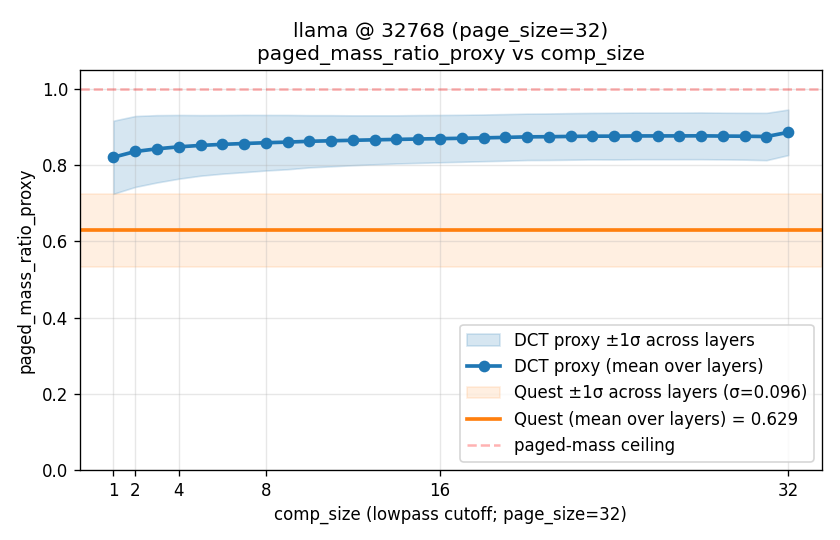
\includegraphics[width=0.85\textwidth]{figures/paged_mass_recall.png}
  \caption[Paged attention-mass recall vs.\ DCT-lowpass cutoff.]
  {Paged attention-mass recall (Eq.~\eqref{eq:mass-recall}) on a
  RULER NIAH-MultiKey~3 trace at $L = 32{,}768$ with
  Llama-3.1-8B-Instruct, page size $P{=}32$, budget $B{=}64$ pages.
  The DCT-lowpass-IDCT proxy of Section~\ref{sec:proxy} (blue)
  routes $\approx 85\%$ of the dense softmax mass to its selected
  pages already at $C{=}4$, with no further gain from increasing
  $C$; the per-channel min/max scorer of Quest (orange) covers only
  $62.9\%$ of the mass at the same budget.  Shaded bands are
  $\pm 1\sigma$ across transformer layers.}
  \label{fig:mass-recall}
\end{figure}

\paragraph{Quantitative comparison.}
At the default DCT-Page configuration of Section~\ref{sec:config}
($C{=}4$, i.e.\ $C/P = 1/8$), the DCT-lowpass-IDCT proxy attains a
paged mass-recall of $84.6\%$ averaged across layers, while Quest's
per-channel min/max statistics cover only $62.9\%$ of the dense
softmax mass at the same per-step budget.  This is a $21.7$-point gap
in the only intermediate quantity that connects scorer geometry to
downstream attention error.  The DCT-Page curve is also remarkably
flat in $C$: doubling the proxy length from $4$ to $32$ buys less than
two points of additional mass-recall, which is consistent with the
spectral concentration documented in Section~\ref{sec:insight} ---
the energetic structure of a page already lives in its first few DCT
bins, and additional bins mostly fit noise.  The flatness in turn
justifies the choice $C{=}4$ as the operating point: it minimizes
proxy-cache footprint and per-page compression cost without giving up
recall.

\paragraph{Implications for downstream accuracy.}
The sparse attention output is a softmax-weighted sum of values, so its
deviation from Full-KV at a single step is upper-bounded by the
softmax mass that the scorer routed \emph{away}, $1 - m(\mathcal{T})$.
DCT-Page misses $\approx 15\%$ of that mass at $C{=}4$; Quest misses
$\approx 37\%$.  This gap is not academic: it is the mechanism behind
the $+5.16$ and $+6.40$-point RULER averages of DCT-Page over Quest
on Llama and Qwen3 reported in Table~\ref{tab:ruler}.  In particular,
the largest per-task gap --- NIAH-MultiKey~3, where DCT-Page reaches
$92.00$ on Llama versus Quest's $32.00$, and $72.00$ on Qwen3 versus
Quest's $8.00$ --- is exactly the task whose dense softmax is the most
concentrated on a single page (the needle's page).  When the dense
distribution is concentrated, missing $37\%$ of its mass is much more
likely to also miss the needle page entirely than missing $15\%$,
which is precisely what the per-task numbers show.


% =====================================================================
\section{Where DCT-Page Wins and Where It Lags}\label{sec:task-level}
% =====================================================================

The headline averages of Chapter~\ref{chap:results} hide a wide
per-task spread.  Reading the rows of Tables~\ref{tab:ruler},
\ref{tab:longbench-v1}, and~\ref{tab:longbench-v2} side by side
reveals two complementary regimes for page-level selection --- one in
which the mass-recall advantage of Section~\ref{sec:mass-recall}
translates almost directly into accuracy, and one in which no
fixed-budget page selector, DCT-Page included, can fully cover what
the task needs.  This section walks through the four most informative
findings.

\subsection{Wins on Retrieval-Style Tasks}\label{sec:wins-retrieval}

The retrieval rows of Table~\ref{tab:ruler} --- NIAH MultiKey,
MultiValue, MultiQuery, and Variable Tracking --- are where the
mass-recall advantage of Figure~\ref{fig:mass-recall} cashes out most
directly.  On Llama-3.1-8B-Instruct, DCT-Page reaches $92.00$ on
NIAH-MultiKey~3 against Quest's $32.00$ (a $60.00$-point gap),
$100.00$ on NIAH-MultiValue against Quest's $97.00$, and $100.00$ on
NIAH-MultiQuery against Quest's $99.00$.  The Qwen3-8B picture is
even sharper: DCT-Page reaches $72.00$ on NIAH-MultiKey~3 against
Quest's $8.00$ (a $64.00$-point gap), $97.00$ on NIAH-MultiValue
against Quest's $90.00$, and $100.00$ on Variable Tracking against
Quest's $98.40$.  On every one of these tasks DCT-Page also matches
or comes within a single point of Full-KV.

These tasks share a common structure: the answer lives at a small
number of identifiable positions, and the dense softmax at the
decode step concentrates sharply on the page(s) holding those
positions.  Page selection therefore reduces to ``find the needle's
page,'' which is exactly what a high-fidelity intermediate
representation of the page should support.  The DCT-lowpass-IDCT
proxy of Section~\ref{sec:proxy} keeps the position-correlated
low-frequency structure of the page and discards only the
high-frequency residual, so the inner product
$q^\top K_p^{\text{proxy}}[c, :]$ remains close to the maximum dense
score $\max_n q^\top K_p[n, :]$ that would have decided whether the
page contains the needle.  Quest's per-channel min/max captures only
the marginal extreme value of each feature dimension and discards the
joint structure across positions inside the page; this is enough for
the easier NIAH variants (single-needle MultiKey~1 and~2) but breaks
down on MultiKey~3, which is the hardest needle-in-needle setting in
the suite.

\subsection{Lags on Word-Frequency and Aggregation Tasks}\label{sec:lags-aggregation}

The Common Words Extraction (CWE) and Frequent Words Extraction (FWE)
rows of Table~\ref{tab:ruler} tell the opposite story.  On Llama,
DCT-Page records $28.00$ on CWE against Quest's $30.00$ and Full-KV's
$48.40$, and $93.33$ on FWE (tied with InfLLM, ahead of Quest's
$82.67$).  On Qwen3 the gap widens: DCT-Page records $46.00$ on CWE
against Quest's $58.80$ and Full-KV's $86.40$, a $12.80$-point loss to
Quest and a $40.40$-point loss to Full-KV.  CWE/FWE are aggregation
tasks --- the model must count words across the entire context and
report the most common --- rather than retrieval tasks.

The dense softmax for an aggregation question is by construction
\emph{not} concentrated on a single page; the relevant evidence is
spread across many pages, and the answer is a function of the broad
distribution rather than of any single peak.  A fixed-budget page
selector restricted to $B{=}64$ pages has no way to integrate the
contributions of the $N - k$ unselected middle pages, and the
per-step error is bounded below by the unrecovered mass however well
the scorer ranks pages.  The fact that Quest is ahead on Qwen3 CWE is
consistent with this picture: when no scorer can route most of the
mass, a coarser but smoother selector that hedges across pages may
edge out a sharper one that commits hard to its top picks.  This is a
\emph{structural} limitation of fixed-budget page selection rather
than a deficiency of the DCT proxy specifically, and it suggests a
direction --- combining page-level top-$k$ with a coarse summary of
the unselected mass --- that we leave to future work.

\subsection{Catastrophic Long-Context Failure of Quest}\label{sec:quest-collapse}

The most dramatic failure mode in Chapter~\ref{chap:results} is
Quest's behaviour on the Long context bucket of LongBench~v2
(Table~\ref{tab:longbench-v2}).  Quest scores $0.00$ on Llama and
$0.93$ on Qwen3 --- effectively random performance below the
four-choice chance level of $25\%$.  DCT-Page, run with the same
$2{,}048$-token selected budget on the same prompts, scores $30.56$
on Llama and $26.85$ on Qwen3, both within $3$ points of Full-KV
($28.70$ and $33.33$ respectively).

We attribute the gap to two compounding properties of the per-channel
min/max scorer.  First, as the number of middle pages $N$ grows with
context length, the per-channel \emph{minimum} and \emph{maximum}
statistics of each page become near-degenerate across pages: at long
context every feature dimension has been driven to nearly the same
extreme values somewhere in almost every page, so the page-to-page
ranking induced by $\max(\,q^\top K^{\min}_p,\, q^\top K^{\max}_p)$
loses discriminative power.  Second, the inner product is taken
against the marginal extremes of $K_p$ independently per channel, so
the score never sees the within-page \emph{co-occurrence} structure
that distinguishes ``the page that contains the answer'' from a
neighbour that shares the same marginal extremes by accident.  On
LongBench~v2 prompts at the Long bucket --- which exceed $32$K
tokens of real text rather than synthetic needles --- both effects
hit simultaneously, and selection essentially stops working.  The
DCT-lowpass-IDCT proxy is by construction sensitive to the
position-correlated low-frequency structure inside each page
(Section~\ref{sec:insight}), and its mass-recall in
Figure~\ref{fig:mass-recall} does not degrade with context length the
way Quest's accuracy does on this benchmark.

\subsection{Sparse Attention Exceeding Full-KV on LongBench v2}\label{sec:lbv2-surprise}

A more subtle phenomenon visible in Table~\ref{tab:longbench-v2} is
that DCT-Page slightly exceeds its own Full-KV baseline on overall
LongBench~v2 accuracy: $30.02$ vs.\ $29.82$ on Llama ($+0.20$) and
$32.01$ vs.\ $29.64$ on Qwen3 ($+2.37$).  SeerAttention-R on Qwen3
shows the same direction at a larger magnitude ($32.60$ vs.\
$29.64$).  A sparse attention method outperforming its own dense
counterpart on a real long-context multiple-choice benchmark is not
what we expected to see, and we do not have a clean explanation;
two interpretations are consistent with the data and we report both.

The first is an implicit-denoising effect.  By zeroing out the
contribution of the $N - k$ unselected middle pages, page-level
top-$k$ selection effectively sharpens the softmax toward the
highest-scoring evidence and suppresses the long tail of low-mass
distractor pages that LongBench~v2 questions are specifically
designed to include.  If a fraction of the dense softmax mass at long
context routes to noise rather than to useful evidence, then removing
it can plausibly improve the model's discrimination among the four
multiple-choice options without changing what the model knows.  The
second is statistical: LongBench~v2 contains $503$ questions, so each
percentage point of overall accuracy corresponds to roughly five
items, and the Qwen3 gap of $+2.37$ points sits within the range that
a different evaluation seed could plausibly produce.  We do not have
a way to fully decouple the two explanations at this benchmark scale,
so we report the result as observed: page-level sparsification at the
$2{,}048$-token budget does not hurt LongBench~v2 overall accuracy
relative to Full-KV, and on Qwen3 it consistently helps by a small
margin.


% =====================================================================
\section{Limitations}\label{sec:limitations}
% =====================================================================

\paragraph{Residual gap to Full-KV.}
DCT-Page is the best page-based method on every aggregate metric
reported in Chapter~\ref{chap:results}, but it is not universally
best.  On Qwen3-8B RULER it trails Full-KV by $5.11$ points
($83.72$ vs.\ $88.83$, Table~\ref{tab:ruler}), and on Qwen3-8B
LongBench~v2 overall accuracy SeerAttention-R edges it out by $0.59$
points ($32.60$ vs.\ $32.01$, Table~\ref{tab:longbench-v2}).  The
RULER gap is concentrated in the aggregation tasks discussed in
Section~\ref{sec:lags-aggregation}, while the SeerAttention-R win is
small enough to fall within the statistical envelope noted in
Section~\ref{sec:lbv2-surprise}; nevertheless, the existence of a gap
to dense attention and the existence of a method that beats DCT-Page
on one benchmark cell are both worth stating plainly.

\paragraph{Decode-only sparsification.}
DCT-Page modifies only the decode path; prefill remains standard
dense attention (Chapter~\ref{chap:method}).  The speedups reported in
Section~\ref{sec:results-speed} therefore apply only to the
autoregressive generation phase, and workloads dominated by
long-prompt prefill --- batch document scoring, long-document
encoders used in a single forward pass, etc.\ --- see no benefit from
the proxy machinery.  This is a deliberate scope choice (the page
proxy is most informative once a query is available to score it
against) but it should be read as a limitation when comparing to
methods that target the prefill side as well.

\paragraph{Evaluation scope.}
The empirical claims of this thesis rest on two open-weight
8B-parameter models (Llama-3.1-8B-Instruct and Qwen3-8B,
Section~\ref{sec:models}) evaluated on a single GPU class (NVIDIA RTX
A6000 with $48$~GiB).  Whether the mass-recall advantage of
Section~\ref{sec:mass-recall} transfers to larger models, to
non-instruction-tuned bases, or to GPUs with different memory and
bandwidth characteristics is an open question.  In particular the
relative weight of the bookkeeping kernels in Table~\ref{tab:per-stage}
will shift with the ratio of attention to MLP work, so the end-to-end
speedup figures should be read as illustrative for the 8B-class regime
rather than as a universal constant.

\paragraph{Structural ceiling on aggregation tasks.}
The shortfall on word-frequency tasks analyzed in
Section~\ref{sec:lags-aggregation} is not addressable by tuning the
DCT proxy alone; it follows from the fixed-budget page-selection
paradigm itself.  Any selector that commits all its budget to $B$
pages cannot represent the long tail of mass that aggregation tasks
distribute across the remaining $N - k$ middle pages.  Closing this
gap likely requires either a coarse summary of the unselected pages
that contributes to the attention output alongside the top-$k$
selection, or a hybrid scheme that combines page-level top-$k$ with a
sparser token-level fallback; both are natural next steps that we do
not evaluate here.
